\chapter{The GAPS experiment} \label{appendixGAPSintro}

%-------------------------------------------------------------------------------
%   The Dark Matter unsolved issue
%-------------------------------------------------------------------------------

\section{The Dark Matter unsolved issue}
The study and understanding of Dark Matter is a broad field of modern physics. Dark Matter is a hypothetical component of matter that, unlike known matter, is unaffected by electromagnetic fields. As a result, it does not absorb, reflect, or emit electromagnetic radiation, making it difficult to detect. This is the origin of the term "Dark Matter". Gravitational effects are the only ones that appear to be related to Dark Matter based on astrophysical observations. In fact, some events are not explainable by the common gravity theories accepted by the scientific community, unless there is more matter than what can be detected through all other physical effects. In the standard Lambda-CDM (Cold Dark Matter) model, based on thg Bang, Dark Matter has to exist because \cite{aramaki_2016_review}:

\begin{itemize}
    \itemsep0em
    \item Galaxies and galaxy clusters could not be created in such a little time starting from the Big Bang calculated instant.
    \item In the present cosmological scenario (that has only the gravity as a cosmological force) galaxies behaviour cannot be explained considering the visible matter only since it is not able to generate sufficient gravitational force.
\end{itemize}

Modern measurements indicate that Dark Matter accounts for \SI{86}{\percent} of the total mass of the universe. Moreover, in the standard Lambda-CDM model, the total mass–energy of the universe is composed of \cite{feng_2010_dark}:

\begin{itemize}
    \itemsep0em
    \item \SI{5}{\percent} ordinary matter and energy,
    \item \SI{26}{\percent} Dark Matter,
    \item \SI{69}{\percent} dark energy.
\end{itemize}

Dark Matter and dark energy are two different concepts. The sum of the Dark Matter and the dark energy account for \SI{95}{\percent} of the total mass–energy content.

%-------------------------------------------------------------------------------

\subsection*{Dark Matter identification}
Another major issue that researchers are attempting to solve is the identification of Dark Matter. Some experiments seek to directly detect Dark Matter, while others seek to detect the byproducts of its self-annihilation or decay. \cite{feng_2010_dark} A brief description of these experiments is presented below.

\begin{itemize}
    \itemsep0em
    \item \textbf{Direct detection experiments}: These experiments attempt to observe the recoils caused by the interaction of Dark Matter passing through the earth with atomic nuclei at very low energies. When Dark Matter passes through special sensitive apparatuses, the particles emit light (scintillators) or phonons (calorimeters). Instruments must be able to differentiate between background particles, which primarily scatter electrons, and Dark Matter particles, which scatter nuclei.
    \item \textbf{Indirect detection experiments}: Experiments of this type attempt to detect the products of self-annihilation or decay of Dark Matter particles in space. In theory, two Dark Matter particles could annihilate in areas with a high density of Dark Matter. In fact, some regions, such as the center of our galaxy, are expected to have a high concentration of Dark Matter. These events are thought to produce gamma rays, Standard Model particle-antiparticle pairs, or Standard Model particles. The main challenge of this type of detection is distinguishing products of Dark Matter annihilation from products of other astrophysical sources \cite{doetinchem_2020_cosmicray}. As a result, different types of evidence are required for a conclusive discovery.
    \item \textbf{Collider searches for Dark Matter}: These experiments attempt to recreate Dark Matter particles in special colliders (like the Large Hadron Collider at CERN in Geneva). All collider discoveries must be validated by further direct or indirect tests to prove that the newly discovered particle is indeed Dark Matter.
\end{itemize}

\noindent
Because of their unusual sensitivity to annihilating and decaying Dark Matter, cosmic-ray antinuclei (antiprotons, antideuterons, and antihelium) can help researchers show or reject a variety of Dark Matter ideas. These indirect detections can also be used to avoid or supplement collider, direct, or other cosmic-ray searches. The hunt for cosmic antideuterons is a novel experiment that provides a strong new approach of studying cosmic physics. The antideuteron is distinguished by its extremely low astrophysical backdrop, particularly at low energies. In reality, some Dark Matter theories anticipate antideuteron flow with energies in the order of a few GeV/n \cite{doetinchem_2020_cosmicray}. All other sorts of Dark Matter searches often attempt to find other types of particles, such as the positron, at greater energy levels (around \SI{100}{\giga\electronvolt}). The key challenge for these tests is distinguishing the results of Dark Matter annihilation from other conventional sources of positrons in this energy range.

%-------------------------------------------------------------------------------
%   The GAPS experiment
%-------------------------------------------------------------------------------

\section{The GAPS experiment}
\label{appendixGAPSexperiment}
The primary goal of the General Antiparticle Spectrometer (GAPS) experiment is the indirect detection of low-energy cosmic-ray antinuclei (below \SI{0.25}{\giga\electronvolt}) \cite{doetinchem_2020_cosmicray}. The experiment consists of 10 layers of semiconducting Si(Li) strip detectors surrounded by a Time Of Flight (TOF) plastic scintillator system on all sides. GAPS is based on a unique particle identification approach based on exotic atom production and decay \cite{re_2022_a}\cite{re_2022_b}. A low-energy antiparticle, slowed by the environment, first travels through the TOF. This enables the collection of preliminary data on particle velocity and energy. When an antiparticle goes through the detector, it loses energy in the Si(Li) detector tracking system and slows down until it stops inside the device. If this occurs, the antiparticle replaces a silicon shell electron, resulting in the formation of an exotic atom in an excited state with a probability close to one. The exotic atom de-excites via auto-ionization and radiative transitions that produce X-rays before annihilating with the silicon nucleus, forming a nuclear star of pions and protons. The antiparticle and silicon decreased mass and atomic numbers determine the X-ray energy in a unique way.

\par
The rejection of the dominating antiproton backdrop is the most difficult challenge in finding antideuterons. The GAPS detector design, on the other hand, allows for the detection of either antiproton or antideuteron cosmic rays. Antihelium signatures can be easily recognised even if the equipment is optimised for antideuteron detection \cite{aramaki_2014_potential}. Because antihelium has a larger charge than antideuterons and antiprotons, its analysis is significantly simpler than the antideuterion-antiproton one.

\begin{figure}[ht]
    \centering
    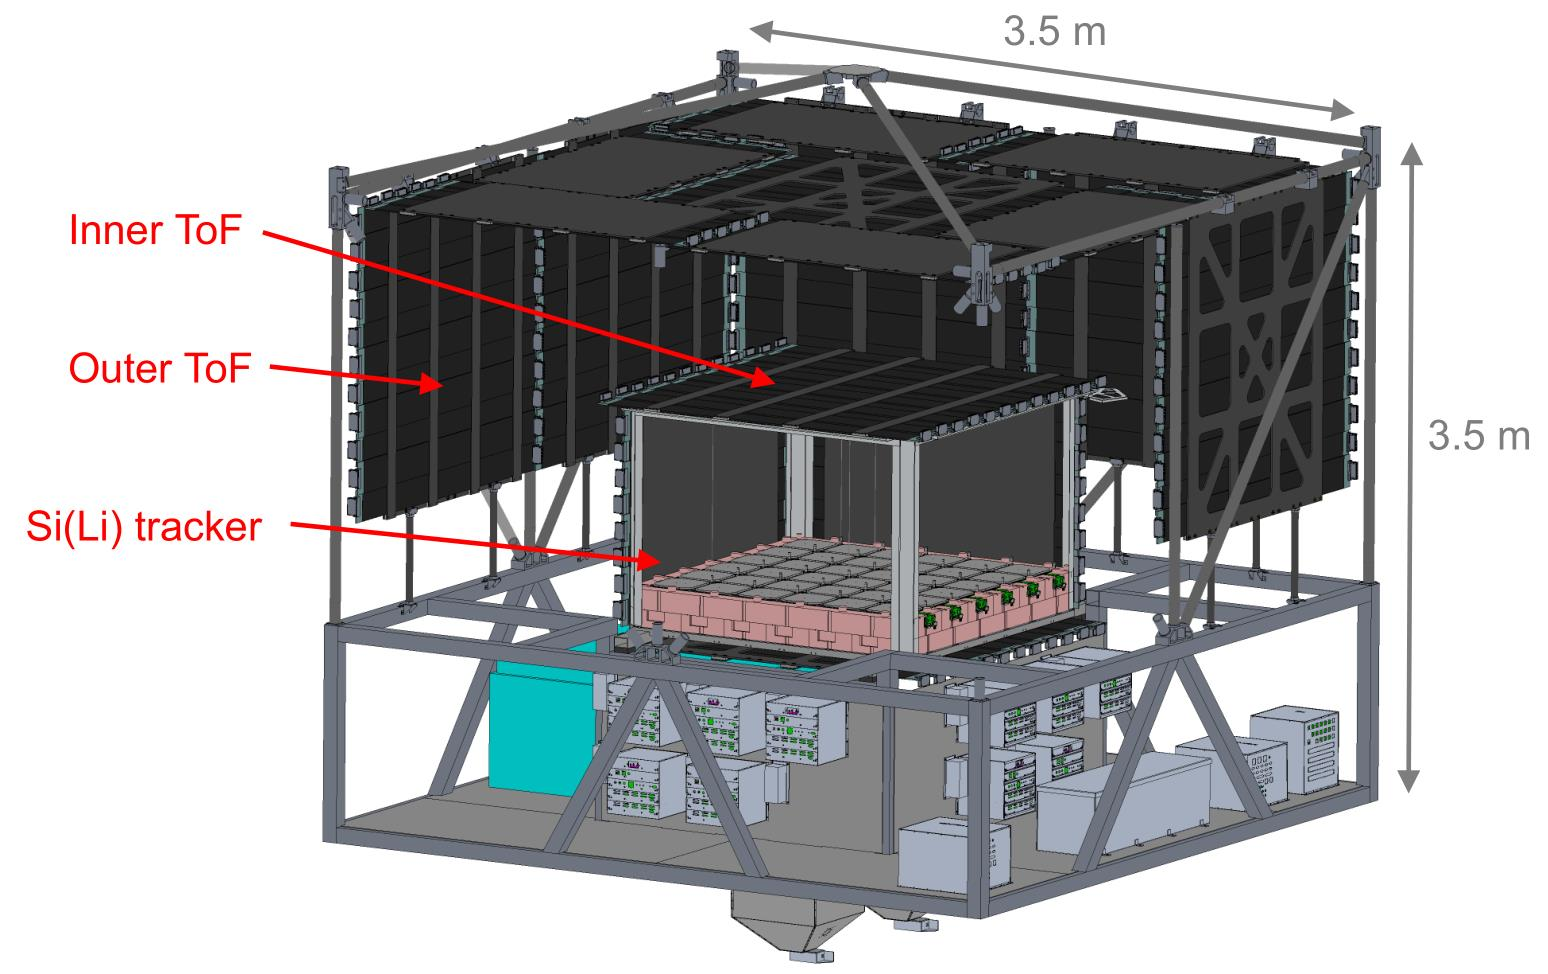
\includegraphics[width=0.9\textwidth]{Images/appendGAPSintro/GAPS_tracker_structure.jpg}
    \caption{Complete GAPS tracking system structure.}
    \label{figGAPStrackerstructure}
\end{figure}

%-------------------------------------------------------------------------------

\subsection*{GAPS tracking system}
\label{gapsTrackingSystem}
The GAPS instrument, shown in \hyperref[figGAPStrackerstructure]{Figure \ref{figGAPStrackerstructure}}, is mainly composed of \cite{rogers_2019_largearea}:

\begin{itemize}
    \itemsep0em
    \item Two external layers of TOF plastic scintillators that surround the inner tracker. The outer TOF dimension are $3.5 \times \SI{3.5}{\metre\squared}$, with an height of \SI{1.5}{\metre}. The inner TOF dimension are $1.5 \times \SI{1.5}{\metre\squared}$, with height of \SI{1}{\metre}. The distance between the outer TOF and the inner TOF is \SI{1}{\metre}. The entire TOF time resolution is about \SI{300}{\pico\second} \cite{doetinchem_2020_cosmicray}.
    \item The inner tracker is subdivided in 10 layers with \SI{10}{\cm} separation in order to achieve 3D particle tracking. Each layer is composed of $12 \times 12$ Si(Li) detectors \cite{spieler_2014_semiconductor}. Each detector has a diameter of \SI{10}{\cm} and a thickness of \SI{2.5}{\mm}. Moreover, each detector is segmented in 8 strips in order to improve the spatial resolution enough to distinguish tracks from incident particles and exotic atom annihilation products. Each strip is then connected to a front-end channel which processes the charge released by the passing particle. The GAPS detectors are capable to detect X-rays ranging from \SI{20}{\kilo\electronvolt} to \SI{80}{\kilo\electronvolt} and charged particles up to \SI{50}{\mega\electronvolt}, at an operating temperature of \SI{-40}{\celsius}, with a FWHM energy resolution lower than \SI{4}{\kilo\electronvolt}. During flight, the cooling operation will be executed by a passive oscillating heat pipe approach, tested on two prototype test flights \cite{okazaki_2014_development}.
    \item Each layer of the inner tracker's circuitry is made up of $6 \times 6$ modules. Each module consists of a readout ASIC and a front-end board. Four detectors are linked to a single module. Each ASIC has 32 front-end channels capable of processing signals from 32 strips. The front-end board contains all of the components required to ensure the ASIC's proper operation. A flex-rigid board, particularly intended for this duty, may link two front-end boards for a total of six front-end boards connected on the same line.
\end{itemize}

%-------------------------------------------------------------------------------
%   GAPS front-end
%-------------------------------------------------------------------------------

\section{GAPS front-end}
\label{secGAPSfrontend}

SLIDER32, the final ASIC for the GAPS experiment, contains 32 channels. Each channel is linked to a different detector strip. When an antiparticle goes through one of the GAPS instrument's strips, it loses energy in each of the Si(Li) detector layers. When it has expended enough energy, it comes to a halt and creates an exotic excited atom. The atom then de-excites and produces X-rays. The nucleus that remains annihilates, producing pions and protons. When an antiparticle travels over a detector strip, it emits a little quantity of charge.

\par
The antiparticle annihilation causes a little quantity of charge to be released in the detector strips. The main purpose of the channel front-end is to analyse the quantity of charge coming from the associated detector strip. This is accomplished by collecting current pulses at the channel's input and turning them into an analog voltage, which is then digitised using an analog-to-digital converter. It is feasible to deduce which particle travelled through the detector based on these digitised values.

\par
The GAPS front-end channel has been designed with a \SI{180}{\nano\meter} CMOS technology and its schematic is shown in \hyperref[figGAPSchannel]{Figure \ref{figGAPSchannel}}. The design has been carried out to target the experiment requirements reported in \hyperref[tabGAPSrequirements]{Table \ref{tabGAPSrequirements}}.

\begin{table}[ht]
    \centering
    %\def\arraystretch{1.3}
    \begin{tabular}{c c} 
         \Xhline{2\arrayrulewidth}
         Requirement & Value \T\B \\
         \hline
         Temperature & \SI{-40}{\celsius} \T\B \\
         Power consumption & < \SI{10}{\milli\watt}/channel \T\B \\
         Input dynamic range & \SI{10}{\kilo\electronvolt} - \SI{50}{\mega\electronvolt} \T\B \\
         Maximum electronic noise interference & \SI{4}{\kilo\electronvolt} (FWHM) \T\B \\
         Minimum threshold & \SI{10}{\kilo\electronvolt} \T\B \\
         Detector leakage current & max \SI{50}{\nano\ampere} @ \SI{27}{\celsius} \T\B \\
         \Xhline{2\arrayrulewidth}
    \end{tabular}
    \caption{GAPS ASIC requirements.}
    \label{tabGAPSrequirements}
\end{table}

%-------------------------------------------------------------------------------

\subsection{Injection circuit}
The injection circuit generates a current pulse, whose amplitude is decided by the user, in order to simulate the release of charge due to the passage of particles through the GAPS Si(Li) detector. This block is used only during the test phase, because in the real experiment, the channels will be connected to the detector strips. 

\par
An injection capacitor $C_{inj}$, shown in \hyperref[figGAPSchannel]{Figure \ref{figGAPSchannel}}, is integrated in each channel to generate the current pulse emulating the charge released in the detector.

\begin{figure}[h!]
    \centering
    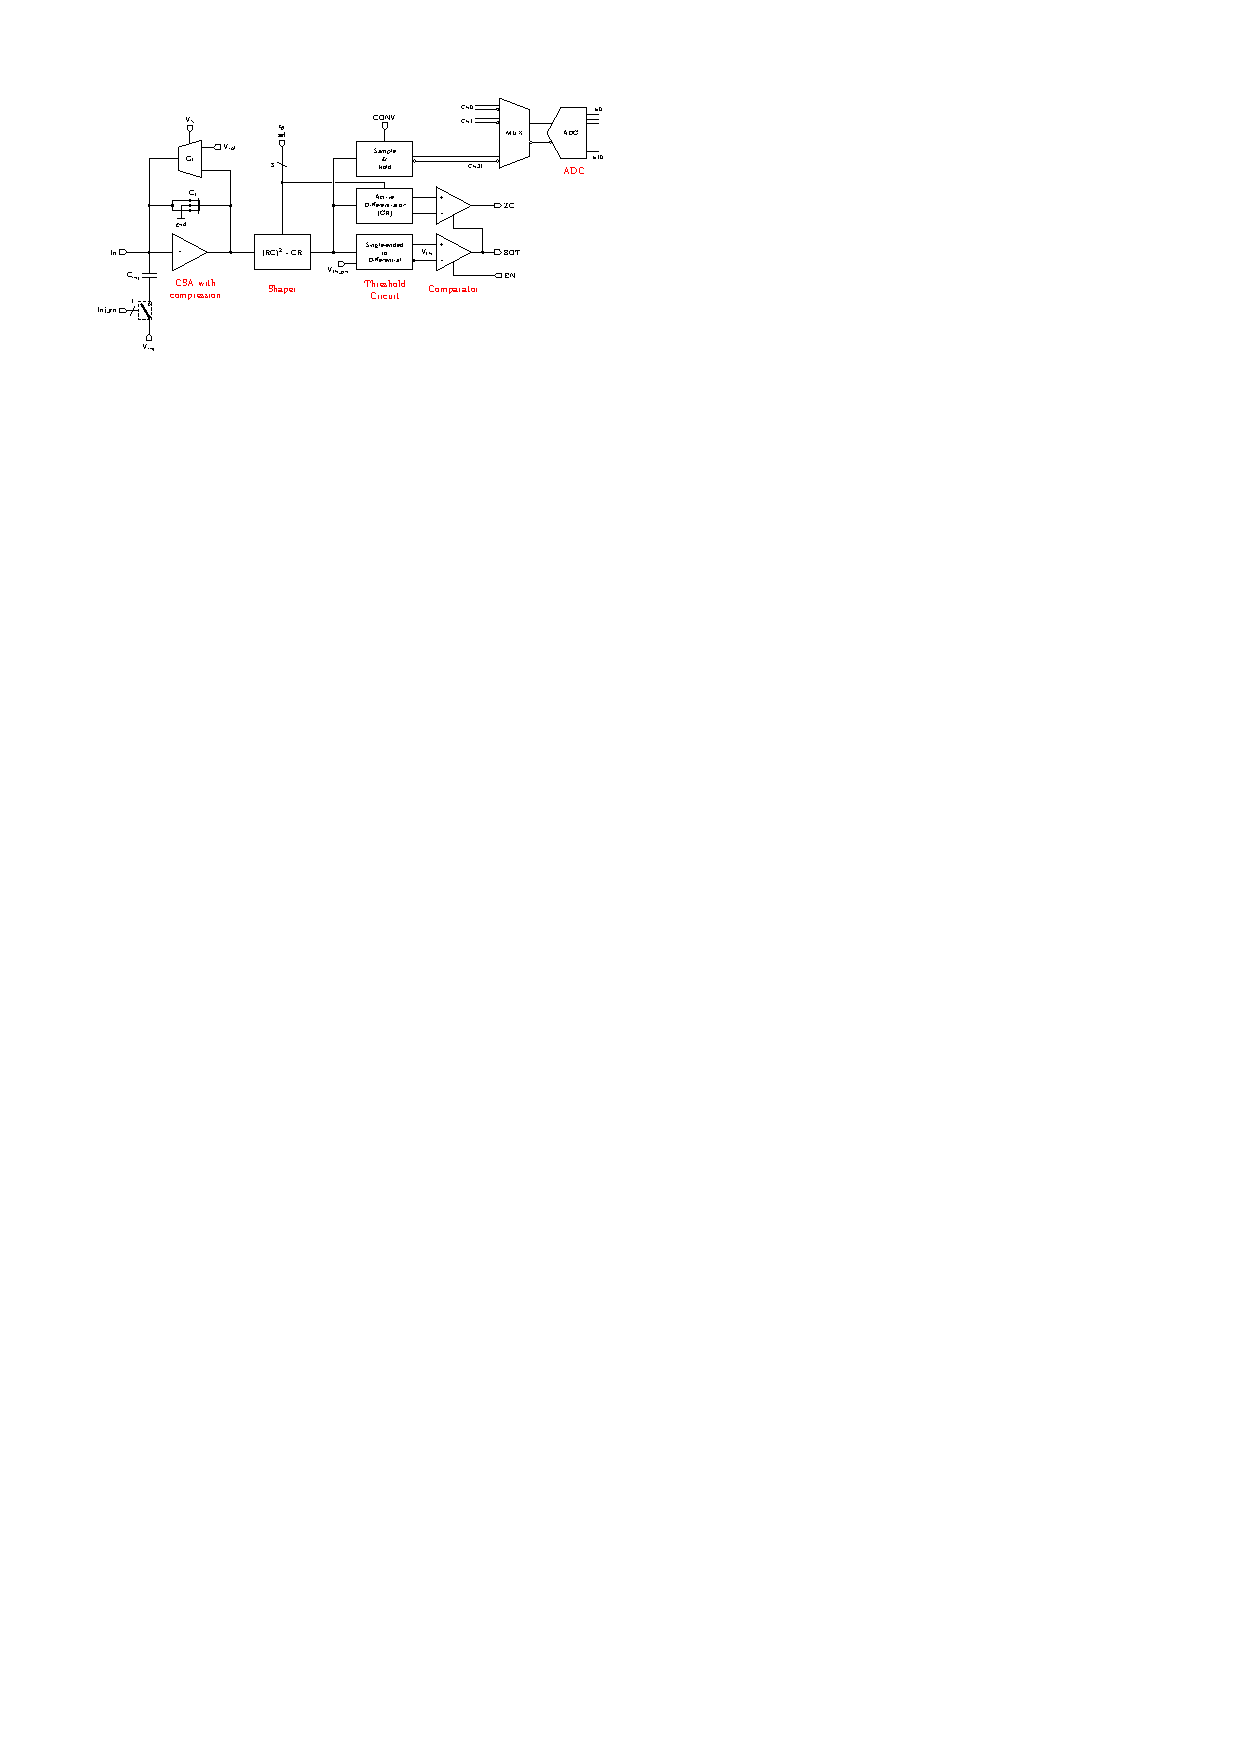
\includegraphics[width=0.98\textwidth]{Images/appendGAPSintro/readoutchannelADC.pdf}
    \caption{Front-end channel schematic.}
    \label{figGAPSchannel}
\end{figure}

%-------------------------------------------------------------------------------

\subsection[Charge Sensitive Amplifier with dynamic signal compression]{Charge Sensitive Amplifier with dynamic signal \\compression}
The Charge Sensitive Amplifier is the channel's initial block. The goal of this block is to transform the detector's current pulses into a voltage step whose amplitude is proportional to the area of the current pulse. This block's key feature is its input-output trans-characteristic, which is defined by  dynamic signal compression. This is a critical feature of the CSA because, due to the high supply voltage and large number of bits required for this solution, a linear gain was not an option for covering the large energy dynamic range required by the project specifications and maintaining a high resolution in the low energy range.

\par
The CSA is built around an active folded cascode (with local feedback) that is loaded using an active cascode architecture. A continuous time feedback implemented using a Krummenacher network does the reset. The dynamic compression has been performed using the nMOS capacitor $C_f$.

%-------------------------------------------------------------------------------

\subsection{Time-invariant filter (CR-(RC)\textsuperscript{2})}
\label{shaper}
The shaper is the second GAPS channel block. The primary purpose of this block is to enhance the Signal-to-Noise ratio in order to achieve the requisite high energy resolution. It consists of two stages: one CR (high-pass filter) and two RC (low-pass filter). This block's Transfer Function is

\begin{equation}
    H(s) = \frac{R_2}{R_1} \cdot \frac{1}{1+s\tau} \cdot \frac{C_2}{C_1} \cdot \frac{s\tau}{(1+s\tau)^2}
\end{equation}

\noindent
The shaper output is a unipolar semi-Gaussian function, characterized by a peaking time $t_p = 2 \cdot \tau$, where $\tau$ is the time constant of the circuit. The peaking time selection (3 bit) is obtained by switching four capacitors. The shaper output introduces a gain of 1.5 almost independent of the peaking time.

%-------------------------------------------------------------------------------

\subsection{Threshold Generator and SOT comparator} \label{thrSOT}
The threshold generator is linked to the shaper output. The remaining two inputs are threshold voltages. This block transforms the single-ended signal from the shaping stage's output to a differential signal. To avoid crosstalk, a differential threshold voltage is utilised. The threshold generator's two output signals are:

\begin{equation}
    V_{th, out1} = v_{s0} + V_{tp} - \frac{V_{sh}}{2}
\end{equation}

\begin{equation}
    V_{th, out2} = v_{s0} + V_{tp} - \frac{V_{sh}}{2}
\end{equation}

\noindent
where $V_{sh}$ is the shaper output voltage and $v_{s0}$ is a threshold generator bias voltage. The differential signal obtained is

\begin{equation}
    \begin{split}
        V_{th, out1} - V_{th, out2} & = (v_{s0} + V_{tp} - \frac{V_{sh}}{2}) - (v_{s0} + V_{tn} + \frac{V_{sh}}{2}) \\
        & = V_{tp} - V_{tn} - V_{sh}
    \end{split}
\end{equation}

The difference $(V_{tp} - V_{tn})$ can be expressed as $V_{th}$, which is the SOT comparator threshold. The two generated voltages are, in fact, connected to the SOT comparator. Its main goal is to suppress false event caused by noise or disturbances. The comparator fires when

\begin{equation}
    V_{th, out2} > V_{th, out1}
\end{equation}

\noindent
or, more easily, when

\begin{equation}
    V_{sh} > V_{th}
\end{equation}

\noindent
$V_{tp}$ and $V_{tn}$ are created via an 8-bit DAC external to the channels of the SLIDER32 ASIC. These voltages are then linked to each channel's threshold generator. To compensate for process parameter fluctuations in each channel threshold, a 3-bit DAC for fine threshold trimming is added to each of these.

%-------------------------------------------------------------------------------

\subsection{Active CR differentiator and Zero Crossing comparator (ZC)}
\label{zeroCrossing}
The differentiator goal is to use a CR filter to extract the shaper output in order to discover the precise shaper peaking moment. When the shaper signal derivative equals zero, the shaper output is at its maximum voltage, i.e. it has reached its peaking time. This block negates the differentiator output and adds a constant voltage of $V_{dd}/2$ to the derivative signal in the process.

This voltage increase avoids the differentiator output from always being \SI{0}{V} if the derivative is less than \SI{0}{V}. This block's output is then linked to the ZC comparator and compared to $V_{dd}/2$ voltage: if it is larger than $V_{dd}/2$, the ZC output becomes a logic 1. This is the point at which the shaper output must be sampled continuously throughout the \texttt{CONV} signal in order to determine the precise injected charge.

\par
The ZC comparator operates only when the SOT comparator voltage is set to logic 1. This is done to readily eliminate erroneous events generated by noise or external disturbances.

%-------------------------------------------------------------------------------

\subsection{Single-ended to differential S\&H}
When the signal \texttt{CONV} changes from logic 0 to logic 1, this block stores the shaper output voltage value. When the front-end is in self-trigger mode, the \texttt{CONV} signal is identical to ZC; however, when it is not in self-trigger mode, the \texttt{CONV} signal must be supplied from an external source.

\par
The sample \& hold output is then connected to a multiplexer, and finally to an ADC used to digitise the voltage stored in it. All the blocks signals are shown in \hyperref[figASICsignals]{Figure \ref{figASICsignals}} for an incoming energy of \SI{100}{\kilo\electronvolt} at \SI{-40}{\celsius}.

\begin{figure}[h!]
    \centering
    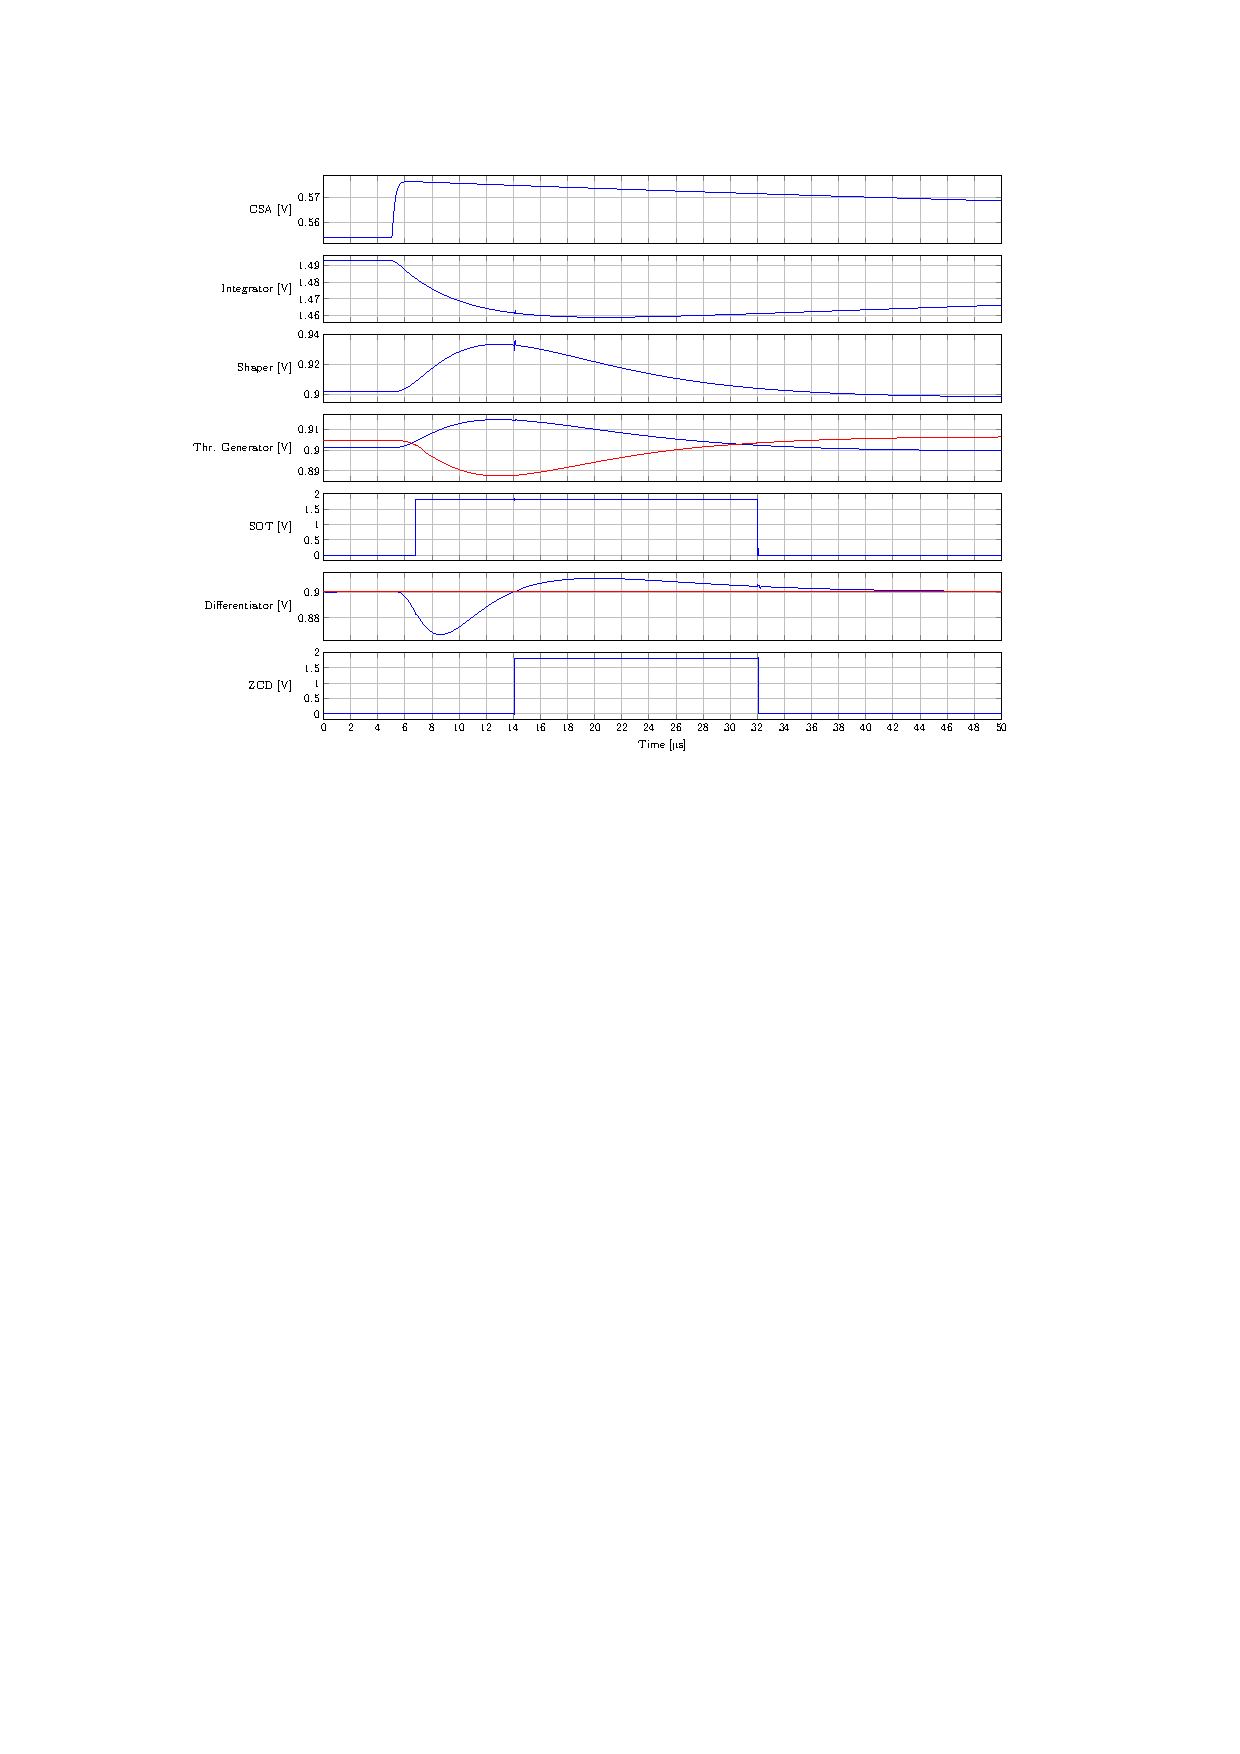
\includegraphics[width=0.99\textwidth]{Images/appendGAPSintro/ASIC_riassunto_segnali.pdf}
    \caption{All channel blocks signals for an incoming energy of \SI{100}{\kilo\electronvolt} at \SI{-40}{\celsius}.}
    \label{figASICsignals}
\end{figure}
